\documentclass[12pt,a4paper]{article}

\usepackage[utf8]{inputenc}
\usepackage[T1]{fontenc}
\usepackage[indonesian, provide=*]{babel}
\usepackage{mathptmx}
\usepackage{geometry}
\usepackage{setspace}
\usepackage{indentfirst}
\usepackage{array}
\usepackage{amsmath}
\usepackage{booktabs}
\usepackage{graphicx}
\usepackage{caption}
\usepackage{longtable}
\usepackage{enumitem}
\usepackage{hyperref}
\usepackage{tikz}
\usetikzlibrary{positioning}

\geometry{left=3cm,right=3cm,top=3cm,bottom=3cm}
\singlespacing
\setlength{\parindent}{1cm}
\setlength{\parskip}{0pt}
\renewcommand{\arraystretch}{1.25}
\renewcommand{\tablename}{Tabel}
\renewcommand{\figurename}{Gambar}
\captionsetup{
  labelsep=space,
  font=normalsize,
  labelfont={},
  textfont={},
  justification=justified,
  singlelinecheck=false
}
\captionsetup[table]{position=above, skip=0pt}
\captionsetup[figure]{position=below, skip=6pt}
\hypersetup{
  colorlinks=true,
  linkcolor=black,
  urlcolor=blue,
  citecolor=black
}

\begin{document}

\pagenumbering{gobble}
\begin{titlepage}
\thispagestyle{empty}
\begin{center}

{\fontsize{14pt}{17pt}\selectfont\bfseries
PROPOSAL PROJECT AKHIR\\
PENGENALAN CITRA DIGITAL
}

\vspace{1.5cm}

{\fontsize{14pt}{17pt}\selectfont\bfseries
KLASIFIKASI STAGE RETINOPATHY OF PREMATURITY\\
BERDASARKAN CITRA FUNDUS BAYI MENGGUNAKAN\\
ENHANCEMENT CITRA, SEGMENTASI PEMBULUH DARAH,\\
DAN CUSTOM CNN
}

\vspace{1.5cm}

{\fontsize{12pt}{14pt}\selectfont
Kelompok 15
}

\vspace{0.5cm}

{\fontsize{12pt}{14pt}\selectfont
\begin{tabular}{ll}
\multicolumn{2}{c}{Anggota Kelompok}\\[0.2cm]
Ghiffari Bravia Hisham & G6401231050 \\
Muhammad Abyan Putra Wibowo & G6401231078 \\
Adam Naufal & G6401231082 \\
Mochamad Chairulridjal Nurvikri & G6401231083 \\
Rafif Muhammad Farras & G6401231102 \\
\end{tabular}
}

\vfill

\includegraphics[width=2.7cm]{../ipb-latex-template/ipb-template-latex/images/ipb_logo.png}

\vfill

{\fontsize{14pt}{17pt}\selectfont\bfseries
PROGRAM STUDI ILMU KOMPUTER\\
FAKULTAS MATEMATIKA DAN ILMU PENGETAHUAN ALAM\\
INSTITUT PERTANIAN BOGOR\\
BOGOR\\
2026
}

\end{center}
\end{titlepage}

\newpage
\pagenumbering{arabic}

\section*{Topik yang Dipilih}

Topik yang dipilih adalah klasifikasi citra medis, dengan kasus khusus klasifikasi stage Retinopathy of Prematurity (ROP) berdasarkan citra fundus bayi. ROP merupakan gangguan perkembangan pembuluh darah retina pada bayi prematur yang dapat menyebabkan gangguan penglihatan serius apabila tidak dideteksi dan ditangani dengan tepat. Pada citra fundus, perubahan struktur retina seperti demarcation line, ridge, area avaskular, serta pola pembuluh darah dapat menjadi petunjuk visual untuk membedakan kondisi normal dan stage ROP.

Topik ini sesuai dengan cakupan project akhir Pengenalan Citra Digital karena sistem yang dibangun tidak hanya melakukan klasifikasi, tetapi juga memuat tahapan pengolahan citra yang eksplisit. Tahapan tersebut meliputi praproses citra, enhancement atau restoration, segmentasi pembuluh darah, ekstraksi fitur citra, pemodelan klasifikasi, dan evaluasi hasil. Citra fundus bayi juga memiliki tantangan nyata, seperti variasi pencahayaan, kontras rendah, blur, area hitam di luar field-of-view retina, serta artefak akibat proses akuisisi citra.

Fokus utama project ini adalah membandingkan pengaruh beberapa representasi citra terhadap performa klasifikasi. Dengan demikian, project tidak hanya mengejar akurasi akhir, tetapi juga menganalisis apakah enhancement citra dan informasi pembuluh darah benar-benar membantu model mengenali stage ROP.

\section*{Dataset yang Dipilih}

Dataset utama yang digunakan adalah dataset dari Zhao et al. (2024), yaitu \textit{A fundus image dataset for intelligent retinopathy of prematurity system}. Dataset ini berisi citra fundus bayi dengan beberapa kategori, yaitu Normal, Stage 1 ROP, Stage 2 ROP, Stage 3 ROP, dan laser scars. Dalam project ini, kelas laser scars tidak digunakan sebagai target utama karena kelas tersebut merepresentasikan kondisi pascaterapi, bukan stage ROP primer.

Ringkasan dataset utama ditunjukkan pada Tabel \ref{tab:dataset-zhao}.

\begin{table}[h]
\centering
\caption{Ringkasan dataset Zhao2024 yang digunakan untuk klasifikasi}
\label{tab:dataset-zhao}
\begin{tabular}{>{\raggedright\arraybackslash}p{4cm} >{\raggedright\arraybackslash}p{8cm}}
\toprule
\textbf{Aspek} & \textbf{Keterangan} \\
\midrule
Nama dataset & A fundus image dataset for intelligent retinopathy of prematurity system \\
Sumber ilmiah & Zhao et al. (2024), Scientific Data \\
Jumlah citra penuh & 1.099 citra fundus dari 483 bayi dan 789 mata \\
Kelas tersedia & Normal, Stage 1, Stage 2, Stage 3, laser scars \\
Kelas yang digunakan & Normal, Stage 1, Stage 2, Stage 3 \\
Kelas yang dikeluarkan & laser scars, karena merupakan kondisi pascaterapi \\
Ukuran citra pada publikasi & Citra diproses menjadi resolusi 512 x 512 \\
\bottomrule
\end{tabular}
\end{table}

Distribusi kelas untuk tugas klasifikasi utama ditunjukkan pada Tabel \ref{tab:kelas}. Setelah kelas laser scars dikeluarkan, total citra yang digunakan adalah 756 citra.

\begin{table}[h]
\centering
\caption{Distribusi kelas untuk klasifikasi Normal dan Stage 1--3}
\label{tab:kelas}
\begin{tabular}{l r}
\toprule
\textbf{Kelas} & \textbf{Jumlah Citra} \\
\midrule
Normal & 236 \\
Stage 1 & 94 \\
Stage 2 & 165 \\
Stage 3 & 261 \\
\midrule
Total & 756 \\
\bottomrule
\end{tabular}
\end{table}

Selain dataset utama, project ini juga menggunakan dataset segmentasi dari Agrawal et al. (2021), yaitu HVDROPDB, sebagai dataset tambahan untuk mengevaluasi kualitas segmentasi pembuluh darah. Bagian yang digunakan terutama adalah citra dan ground truth mask pembuluh darah pada folder HVDROPDB-BV. Ground truth tersebut diperlakukan sebagai binary mask sehingga hasil segmentasi dapat dievaluasi menggunakan metrik seperti Dice, IoU, sensitivity, specificity, dan accuracy.

\section*{Strategi Pembagian Data}

Pembagian data klasifikasi mengikuti rasio yang digunakan pada Zhao et al. (2024), yaitu 8:1:1 untuk train, validation, dan test. Untuk setup empat kelas tanpa laser scars, pembagian yang ditargetkan ditunjukkan pada Tabel \ref{tab:split}.

\begin{table}[h]
\centering
\caption{Rencana pembagian data berdasarkan rasio Zhao2024}
\label{tab:split}
\begin{tabular}{l r r r r}
\toprule
\textbf{Kelas} & \textbf{Train} & \textbf{Validation} & \textbf{Test} & \textbf{Total} \\
\midrule
Normal & 188 & 24 & 24 & 236 \\
Stage 1 & 75 & 9 & 10 & 94 \\
Stage 2 & 132 & 16 & 17 & 165 \\
Stage 3 & 208 & 26 & 27 & 261 \\
\midrule
Total & 603 & 75 & 78 & 756 \\
\bottomrule
\end{tabular}
\end{table}

Split dilakukan secara stratified agar proporsi kelas tetap terjaga pada setiap subset. Namun, dataset lokal tidak menyediakan ID pasien atau ID mata pada nama file. Karena itu, split yang dilakukan berpotensi bersifat image-level, bukan patient-level. Hal ini dapat menimbulkan risiko data leakage apabila beberapa citra dari bayi atau mata yang sama berada pada subset yang berbeda. Risiko ini akan dinyatakan sebagai keterbatasan evaluasi. Apabila metadata pasien atau mata tersedia pada tahap lanjutan, split akan diperbaiki menjadi group-stratified split berdasarkan ID pasien atau ID mata.

\section*{Pipeline Project}

Pipeline umum project ditunjukkan pada Gambar \ref{fig:pipeline}. Pipeline disusun agar memenuhi struktur minimum project akhir, yaitu akuisisi dataset, praproses, enhancement/restoration, segmentasi area penting, ekstraksi fitur, klasifikasi, evaluasi performa, dan analisis hasil.

\begin{figure}[h]
\centering
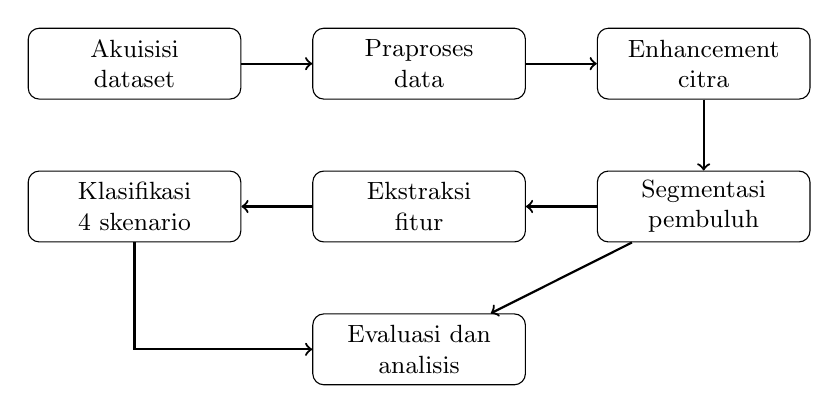
\begin{tikzpicture}[
  node distance=0.9cm,
  every node/.style={draw, rounded corners, align=center, font=\small, minimum width=2.7cm, minimum height=0.9cm},
  arrow/.style={->, thick}
]
\node (data) {Akuisisi\\dataset};
\node (pre) [right=of data] {Praproses\\data};
\node (enh) [right=of pre] {Enhancement\\citra};
\node (seg) [below=of enh] {Segmentasi\\pembuluh};
\node (feat) [left=of seg] {Ekstraksi\\fitur};
\node (cls) [left=of feat] {Klasifikasi\\4 skenario};
\node (eval) [below=of feat] {Evaluasi dan\\analisis};

\draw[arrow] (data) -- (pre);
\draw[arrow] (pre) -- (enh);
\draw[arrow] (enh) -- (seg);
\draw[arrow] (seg) -- (feat);
\draw[arrow] (feat) -- (cls);
\draw[arrow] (cls) |- (eval);
\draw[arrow] (seg) -- (eval);
\end{tikzpicture}
\caption{Alur umum pipeline project dari dataset hingga evaluasi.}
\label{fig:pipeline}
\end{figure}

\subsection*{1. Akuisisi dan Pemahaman Dataset}

Tahap pertama adalah membaca struktur folder dataset Zhao2024, memetakan nama folder menjadi label kelas, dan menghitung distribusi data. Kelas laser scars dikeluarkan dari eksperimen utama. Setelah itu, data dibagi menjadi train, validation, dan test dengan split stratified sesuai rencana pada Tabel \ref{tab:split}. Tahap ini juga mencakup pemeriksaan contoh visual tiap kelas untuk memahami karakteristik citra, variasi orientasi, kualitas pencahayaan, dan potensi kemiripan antar kelas.

\subsection*{2. Praproses Data}

Praproses awal dilakukan secara konsisten untuk seluruh skenario. Setiap citra dibaca sebagai citra RGB, di-resize ke ukuran input model, dan dinormalisasi. Augmentasi ringan hanya diterapkan pada data training, seperti rotasi kecil, flipping jika masih masuk akal secara klinis, serta variasi kecil brightness atau contrast. Augmentasi tidak dibuat agresif karena fitur stage ROP seperti demarcation line dan ridge dapat bersifat halus.

\subsection*{3. Enhancement Citra untuk Klasifikasi}

Enhancement citra untuk klasifikasi mengacu pada gagasan Rahim et al. (2024). Rahim et al. menunjukkan bahwa enhancement berbasis restoration dan CLAHE dapat membantu memperjelas struktur penting pada citra ROP, terutama demarcation line dan ridge. Namun, dataset Rahim et al. berbeda dari dataset Zhao2024. Oleh karena itu, project ini tidak menganggap enhancement pasti meningkatkan performa, tetapi menjadikannya sebagai salah satu skenario eksperimen.

Metode yang digunakan adalah pendekatan konservatif yang terinspirasi dari Rahim et al. Alur yang direncanakan adalah:

\begin{enumerate}[label=\alph*.]
  \item koreksi illumination atau background normalization untuk mengurangi pencahayaan tidak merata,
  \item CLAHE pada kanal luminance di ruang warna LAB atau pada kanal RGB,
  \item denoising ringan apabila diperlukan,
  \item menghasilkan citra RGB enhanced untuk klasifikasi.
\end{enumerate}

Dengan demikian, enhancement yang digunakan dapat dijelaskan sebagai Rahim-inspired enhancement, bukan reproduksi penuh DPFRr. Hasil visual sebelum dan sesudah enhancement akan ditampilkan untuk melihat apakah enhancement memperjelas struktur retina atau justru menimbulkan artefak.

\subsection*{4. Segmentasi Pembuluh Darah}

Segmentasi pembuluh darah mengacu pada pipeline Almeida et al. (2024). Tujuan tahap ini adalah menghasilkan mask pembuluh darah yang dapat digunakan dalam skenario vessel-only dan vessel-guided classification. Alur segmentasi yang direncanakan ditunjukkan pada Gambar \ref{fig:vessel}.

\begin{figure}[h]
\centering
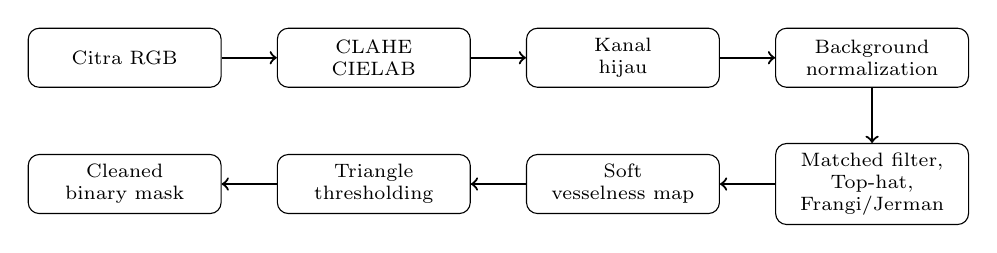
\begin{tikzpicture}[
  node distance=0.7cm,
  every node/.style={draw, rounded corners, align=center, font=\scriptsize, minimum width=2.45cm, minimum height=0.75cm},
  arrow/.style={->, thick}
]
\node (rgb) {Citra RGB};
\node (lab) [right=of rgb] {CLAHE\\CIELAB};
\node (green) [right=of lab] {Kanal\\hijau};
\node (norm) [right=of green] {Background\\normalization};
\node (enhance) [below=of norm] {Matched filter,\\Top-hat,\\Frangi/Jerman};
\node (soft) [left=of enhance] {Soft\\vesselness map};
\node (bin) [left=of soft] {Triangle\\thresholding};
\node (clean) [left=of bin] {Cleaned\\binary mask};

\draw[arrow] (rgb) -- (lab);
\draw[arrow] (lab) -- (green);
\draw[arrow] (green) -- (norm);
\draw[arrow] (norm) -- (enhance);
\draw[arrow] (enhance) -- (soft);
\draw[arrow] (soft) -- (bin);
\draw[arrow] (bin) -- (clean);
\end{tikzpicture}
\caption{Rencana pipeline segmentasi pembuluh darah berbasis pengolahan citra.}
\label{fig:vessel}
\end{figure}

Pipeline menghasilkan soft vesselness map sebagai output antara. Soft map ini berisi nilai kontinu yang menunjukkan kemungkinan suatu piksel merupakan pembuluh darah. Soft map kemudian diubah menjadi binary mask menggunakan Triangle thresholding, lalu dibersihkan dengan postprocessing seperti penghapusan connected component kecil, morphological opening, atau hole filling jika diperlukan. Hasil akhir tahap ini adalah cleaned binary vessel mask.

Ground truth dari HVDROPDB diperlakukan sebagai binary mask. Jika ada file ground truth lokal yang memiliki nilai grayscale karena anti-aliasing atau artefak ekspor, mask tersebut akan dibinarisasi sebelum evaluasi. Evaluasi segmentasi dilakukan antara cleaned binary prediction dan binary ground truth.

\subsection*{5. Ekstraksi Fitur}

Ekstraksi fitur dilakukan melalui dua bentuk representasi. Pertama, fitur eksplisit dari pengolahan citra, yaitu vesselness map dan binary vessel mask yang merepresentasikan struktur pembuluh darah. Kedua, fitur otomatis yang dipelajari CNN dari citra input. Pada CNN, convolutional layer awal mempelajari fitur tepi, tekstur, dan kontras lokal, sedangkan residual block yang lebih dalam mempelajari representasi yang lebih abstrak untuk membedakan Normal, Stage 1, Stage 2, dan Stage 3.

Pada skenario vessel-only, model hanya menerima informasi bentuk dan distribusi pembuluh darah. Pada skenario vessel-guided, informasi pembuluh darah dimasukkan melalui proses masking citra, bukan melalui perubahan arsitektur model.

\subsection*{6. Skenario Klasifikasi}

Empat skenario klasifikasi yang akan dibandingkan ditunjukkan pada Tabel \ref{tab:skenario}. Semua skenario menggunakan split data yang sama agar perbandingan adil.

\begin{table}[h]
\centering
\caption{Empat skenario klasifikasi yang dibandingkan}
\label{tab:skenario}
\begin{tabular}{>{\raggedright\arraybackslash}p{2cm} >{\raggedright\arraybackslash}p{5cm} >{\raggedright\arraybackslash}p{6cm}}
\toprule
\textbf{Skenario} & \textbf{Input} & \textbf{Tujuan Analisis} \\
\midrule
S1 & Citra RGB mentah & Baseline tanpa enhancement \\
S2 & Citra RGB hasil enhancement & Menguji pengaruh enhancement konservatif terinspirasi Rahim et al. \\
S3 & Cleaned binary vessel mask & Menguji apakah struktur pembuluh saja cukup informatif untuk stage ROP \\
S4 & Citra enhanced RGB dengan vessel-guided soft masking & Menguji apakah informasi pembuluh dapat membantu jika dimasukkan sebagai proses pengolahan citra \\
\bottomrule
\end{tabular}
\end{table}

Untuk S4, binary vessel mask tidak digunakan sebagai hard mask langsung karena dapat menghapus konteks retina yang masih penting untuk stage classification. Sebaliknya, cleaned binary mask diubah menjadi soft guide melalui dilation dan Gaussian blur. Contoh formulanya adalah:

\[
\text{guide} = 0.5 + 0.5 \times \text{GaussianBlur}(\text{Dilate}(\text{mask}))
\]

\[
\text{S4 image} = \text{enhanced RGB} \times \text{guide}
\]

Dengan cara ini, area pembuluh dan sekitarnya ditegaskan, tetapi area non-pembuluh tidak dihilangkan sepenuhnya. Output S4 tetap berupa citra RGB tiga kanal sehingga fokus tetap berada pada pengolahan citra, bukan konfigurasi model khusus.

\subsection*{7. Model Klasifikasi}

Model utama yang digunakan adalah custom Tiny ResNet. Model ini dipilih karena dataset relatif kecil sehingga model yang terlalu besar dapat lebih mudah overfit. Tiny ResNet juga cukup sederhana untuk dijelaskan sebagai CNN manual, tetapi tetap memiliki residual connection agar proses training lebih stabil.

Rancangan umum Tiny ResNet adalah:

\begin{itemize}
  \item convolution 3 x 3 dengan 32 filter,
  \item dua residual block dengan 32 filter,
  \item dua residual block dengan 64 filter dan downsampling,
  \item dua residual block dengan 128 filter dan downsampling,
  \item dua residual block dengan 256 filter dan downsampling,
  \item global average pooling,
  \item dropout,
  \item dense layer softmax dengan 4 kelas.
\end{itemize}

Tiny ResNet digunakan pada seluruh skenario S1 sampai S4. Untuk S1, S2, dan S4, input berupa citra RGB tiga kanal. Untuk S3, input berupa binary vessel mask satu kanal.

Sebagai baseline opsional, ResNet50 digunakan hanya pada skenario S1 dan S2. Pembatasan ini dilakukan karena ResNet50 secara natural menerima input RGB tiga kanal dan Zhao et al. (2024) juga melaporkan ResNet50 sebagai model terbaik pada evaluasi dataset mereka. ResNet50 tidak digunakan pada S3 dan S4 agar baseline tetap sederhana dan fokus pada perbandingan raw RGB versus enhanced RGB.

\section*{Strategi Training dan Imbalance Handling}

Dataset memiliki distribusi kelas yang tidak seimbang, terutama karena Stage 1 hanya memiliki 94 citra. Untuk mengurangi dampak imbalance, project ini menggunakan tiga strategi:

\begin{enumerate}[label=\alph*.]
  \item stratified split agar proporsi kelas pada train, validation, dan test tetap terjaga,
  \item class-weighted cross entropy agar kesalahan pada kelas minoritas diberi penalti lebih besar,
  \item evaluasi menggunakan macro precision, macro recall, dan macro F1-score, bukan hanya accuracy.
\end{enumerate}

Optimizer awal yang direncanakan adalah AdamW dengan learning rate sekitar \(10^{-3}\). Model terbaik dipilih berdasarkan macro F1-score pada validation set. Early stopping digunakan untuk mengurangi risiko overfitting.

\section*{Evaluasi Performa}

Evaluasi dilakukan pada dua bagian, yaitu evaluasi segmentasi pembuluh darah dan evaluasi klasifikasi stage ROP.

\subsection*{Evaluasi Segmentasi}

Evaluasi segmentasi dilakukan pada dataset HVDROPDB-BV dari Agrawal et al. (2021). Metrik yang digunakan adalah:

\begin{itemize}
  \item Dice coefficient,
  \item Intersection over Union (IoU),
  \item sensitivity,
  \item specificity,
  \item accuracy.
\end{itemize}

Selain metrik numerik, hasil visual juga disimpan dalam bentuk citra asli, soft vesselness map, cleaned binary vessel mask, dan overlay mask pada citra asli. Visualisasi ini penting untuk mengetahui apakah segmentasi menghasilkan noise, artefak optic disc, atau kehilangan pembuluh halus.

\subsection*{Evaluasi Klasifikasi}

Evaluasi klasifikasi dilakukan pada test set yang sama untuk semua skenario. Metrik yang digunakan ditunjukkan pada Tabel \ref{tab:evaluasi}.

\begin{table}[h]
\centering
\caption{Rencana metrik evaluasi klasifikasi}
\label{tab:evaluasi}
\begin{tabular}{>{\raggedright\arraybackslash}p{4cm} >{\raggedright\arraybackslash}p{9cm}}
\toprule
\textbf{Metrik} & \textbf{Tujuan Penggunaan} \\
\midrule
Accuracy & Memberikan gambaran umum proporsi prediksi benar \\
Macro precision & Mengukur ketepatan prediksi dengan bobot seimbang antar kelas \\
Macro recall & Mengukur kemampuan model mengenali tiap kelas secara seimbang \\
Macro F1-score & Metrik utama untuk membandingkan skenario karena data tidak seimbang \\
Per-class recall & Mengetahui kelas mana yang sulit dikenali, terutama Stage 1 \\
Confusion matrix & Melihat pola kesalahan antar kelas, misalnya Stage 1 tertukar dengan Stage 2 \\
ROC-AUC one-vs-rest & Metrik tambahan apabila diperlukan untuk melihat kualitas skor probabilitas \\
\bottomrule
\end{tabular}
\end{table}

Tabel hasil akhir yang direncanakan ditunjukkan pada Tabel \ref{tab:hasil}.

\begin{table}[h]
\centering
\caption{Template perbandingan hasil empat skenario}
\label{tab:hasil}
\begin{tabular}{l r r r r}
\toprule
\textbf{Skenario} & \textbf{Accuracy} & \textbf{Macro Precision} & \textbf{Macro Recall} & \textbf{Macro F1} \\
\midrule
S1 Raw RGB & TBD & TBD & TBD & TBD \\
S2 Enhanced RGB & TBD & TBD & TBD & TBD \\
S3 Vessel mask & TBD & TBD & TBD & TBD \\
S4 Vessel-guided enhanced & TBD & TBD & TBD & TBD \\
\bottomrule
\end{tabular}
\end{table}

\section*{Analisis yang Direncanakan}

Analisis hasil tidak hanya berfokus pada akurasi akhir. Beberapa pertanyaan utama yang akan dibahas adalah:

\begin{enumerate}
  \item Apakah enhancement konservatif meningkatkan performa dibanding citra mentah?
  \item Kelas mana yang paling terbantu oleh enhancement?
  \item Apakah vessel mask saja cukup untuk membedakan Normal dan Stage 1--3?
  \item Apakah vessel-guided masking meningkatkan performa dibanding enhanced RGB biasa?
  \item Kelas mana yang paling sering tertukar pada confusion matrix?
  \item Apakah Stage 1 sulit dikenali karena demarcation line yang halus?
  \item Apakah kualitas segmentasi pembuluh membatasi performa S3 dan S4?
  \item Apakah Tiny ResNet cukup kompetitif dibanding ResNet50 pada skenario RGB S1 dan S2?
\end{enumerate}

Ekspektasi awal adalah S2 dapat lebih baik dari S1 apabila enhancement berhasil memperjelas struktur retina. S4 juga diharapkan dapat membantu apabila vessel-guided masking menekankan area informatif tanpa menghapus konteks penting. Namun, hasil tersebut hanya hipotesis. Jika enhancement atau vessel-guided masking justru menurunkan performa, hasil tersebut tetap penting karena menunjukkan bahwa metode enhancement dari dataset lain belum tentu langsung cocok untuk Zhao2024.

\section*{Kelemahan dan Risiko Project}

Beberapa kelemahan dan risiko yang perlu dicatat adalah:

\begin{itemize}
  \item jumlah data relatif kecil, terutama pada kelas Stage 1,
  \item split berpotensi image-level karena ID pasien atau ID mata tidak tersedia pada nama file lokal,
  \item label stage ROP dapat bersifat subjektif, terutama pada batas Stage 1 dan Stage 2,
  \item enhancement yang terinspirasi Rahim et al. berasal dari dataset berbeda sehingga transfer ke Zhao2024 belum pasti,
  \item segmentasi pembuluh berbasis pengolahan citra klasik dapat sensitif terhadap kualitas citra dan artefak,
  \item hasil project belum dapat diklaim sebagai validasi klinis karena evaluasi masih terbatas pada dataset publik.
\end{itemize}

\section*{Rencana Kerja}

Rencana pengerjaan project selama empat minggu ditunjukkan pada Tabel \ref{tab:jadwal}.

\begin{table}[h]
\centering
\caption{Rencana pengerjaan project}
\label{tab:jadwal}
\begin{tabular}{>{\raggedright\arraybackslash}p{3cm} >{\raggedright\arraybackslash}p{10cm}}
\toprule
\textbf{Minggu} & \textbf{Kegiatan} \\
\midrule
Minggu 1 & Audit dataset, hitung distribusi kelas, buat split data, dan implementasi baseline raw RGB \\
Minggu 2 & Implementasi enhancement konservatif terinspirasi Rahim et al. dan segmentasi pembuluh darah terinspirasi Almeida et al. \\
Minggu 3 & Evaluasi segmentasi pada HVDROPDB, training Tiny ResNet untuk S1--S4, dan training ResNet50 opsional untuk S1--S2 \\
Minggu 4 & Analisis hasil, confusion matrix, visualisasi failure case, penyusunan laporan, slide, dan demo program \\
\bottomrule
\end{tabular}
\end{table}

\section*{Pustaka}

Agrawal R, Kulkarni S, Walambe R, Kotecha K. 2021. Assistive framework for automatic detection of all the zones in retinopathy of prematurity using deep learning. \textit{Journal of Digital Imaging}. 34:932--947. doi:10.1007/s10278-021-00477-8.

Almeida J, Kubicek J, Penhaker M, Cerny M, Augustynek M, Varysova A, Bansal A, Timkovic J. 2024. Enhancing ROP plus form diagnosis: An automatic blood vessel segmentation approach for newborn fundus images. \textit{Results in Engineering}. 24:103054. doi:10.1016/j.rineng.2024.103054.

Rahim S, Sabri K, Ells A, Wassyng A, Lawford M, He W, Chu L. 2024. Image pre-processing for improving deep learning classification of retinopathy of prematurity. arXiv:2302.02524.

Vahidmoghadam M, Ghorbani P, Ahmadi MJ, Asadi Khameneh E, Tavassoli B, Taghirad HD. 2026. Automated diagnosis of plus form and early stages of ROP using deep learning models. \textit{Scientific Reports}. 16:7234. doi:10.1038/s41598-026-37064-2.

Zhao X, Chen S, Zhang S, Liu Y, Hu Y, Yuan D, Xie L, Luo X, Zheng M, Tian R, Chen Y, Tan T, Yu Z, Sun Y, Wu Z, Zhang G. 2024. A fundus image dataset for intelligent retinopathy of prematurity system. \textit{Scientific Data}. 11:543. doi:10.1038/s41597-024-03362-5.

\end{document}
